\section{Web UI Design}

\textbf {User interface} (UI) design is targeted to let readers use the ScholarHub software conveniently. The UI should be simple and functional to attract the reader’s attention and interests. The UI should avoid being overly complex so that it can be used without learning. The UI of ScholarHub consists of 7 parts. They are explained as follow:

\textbf {Homepage:} there is a logo in the middle to indicate the service function and enhance recognition. A motto at the bottom to inspire academic pursuits. To continue using the service, the user must log in by clicking the “login” button at the top right corner.


\begin{figure}[htbp]
	\centering
	\begin{minipage}[t]{0.48\textwidth}
		\centering
		
\includegraphics[width=6cm]{./img/UI Home page.jpg}
		\caption{Home Page UI}
	\end{minipage}
	\begin{minipage}[t]{0.48\textwidth}
		\centering
		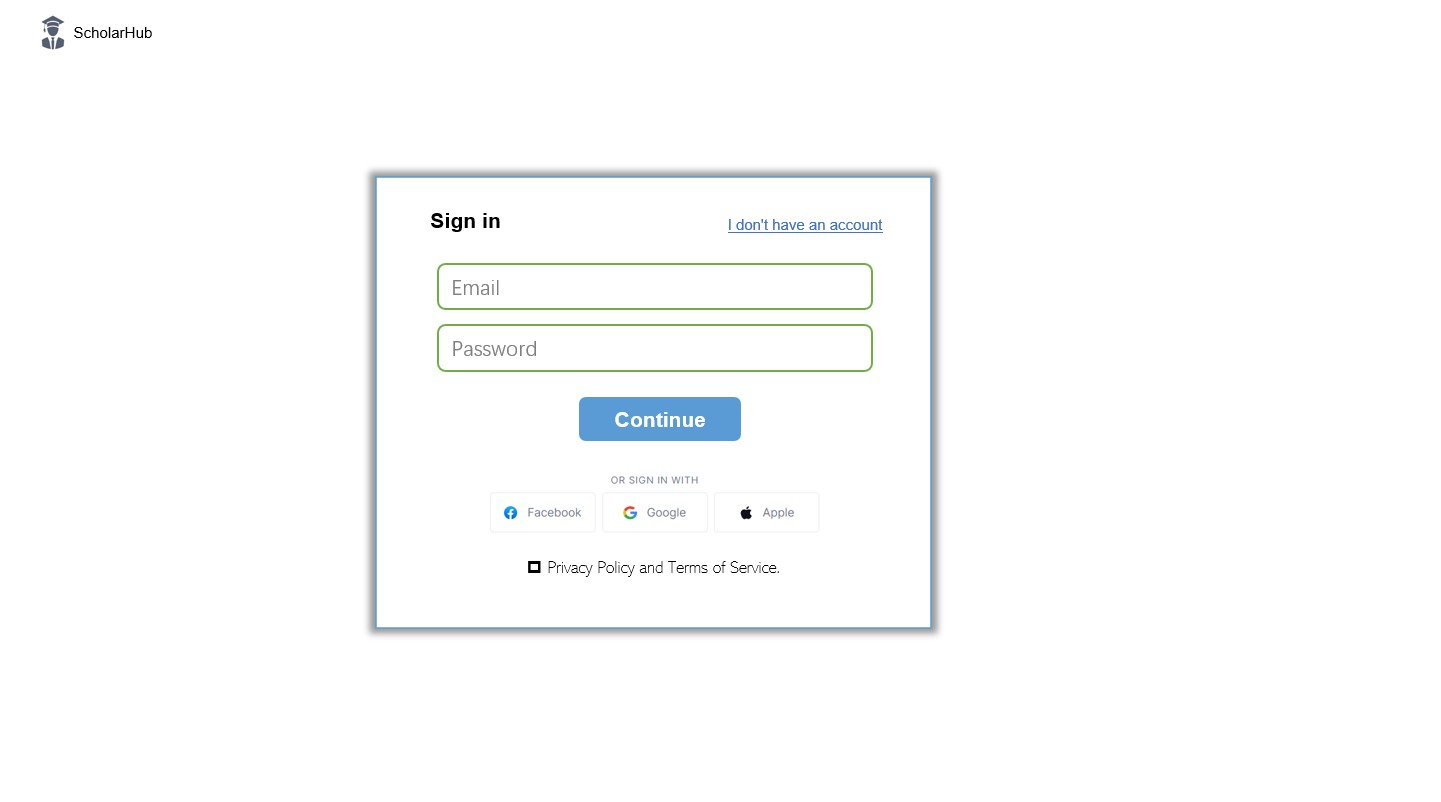
\includegraphics[width=6cm]{./img/UI sign in.jpg}
		\caption{Sign in UI}
	\end{minipage}
\end{figure}

\textbf {Sign in:} Email address and password are required to sign in. if the user does not have an account. It can jump to the registration page by simply clicking “I don’t have an account”. Only Email addresses and Passwords are requested for registration. Additionally, users can log in by connecting with Facebook, Google and Apple.

\textbf {Menu page:} As soon as the user logged in, the web will show the Menu page initially. On the top left is the logo of ScholarHub. Following with four card buttons on the top, which are Menu, Team, My Library and My Profile. These are four main functional pages. On the top middle, there is a search bar, users can search paper titles and team members’ names to directly check the information. On the top right-hand side, the button shows the user’s name to remind it has been login with the current account. The log-out function is inside the name button. The Menu page indicates three main zones. On the left is the team zone, it shows the list of the team that the user joined. In the middle, there is a brief reading list of history. That is for reminding the user to review the recent paper. On the right side is the recent activities zone, users can get go through other team members' activities.

\begin{figure*}[htp]
	\centering
	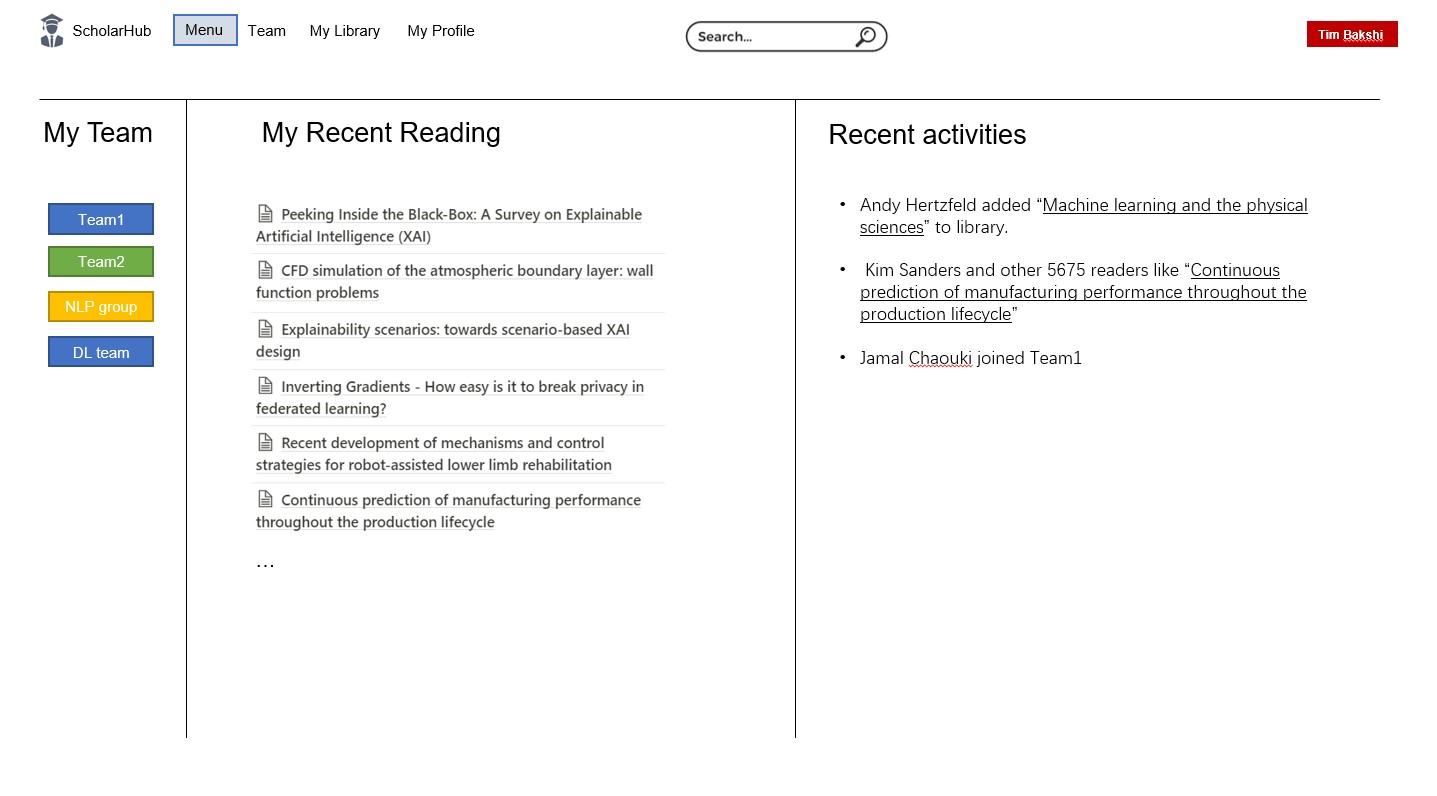
\includegraphics[width=\textwidth]{./img/UI MainPage.jpg}
	\caption{Menu Page UI}
	\label{fig:Memu Page}
\end{figure*}

\textbf {My Library:} this is the main functional page for users to collect and organize their reading list. The list contains the information of Paper title, Authors, Author’s affiliation, Research field tag, Published year, Priority defined by the user, Read checkbox, Like checkbox, Link or DOI of the paper. Finally, the number of likes about the current paper in the system can be shown to the customer. Users can also open a text box and write a note by clicking the paper title. Users can click and check the read and like check-box to remind themselves. Also, the activity will be recorded and collected. This information will be available to the teammates and supervisor. The number of likes by all users will be counted and anonymously shown to others.

\begin{figure*}[htp]
	\centering
	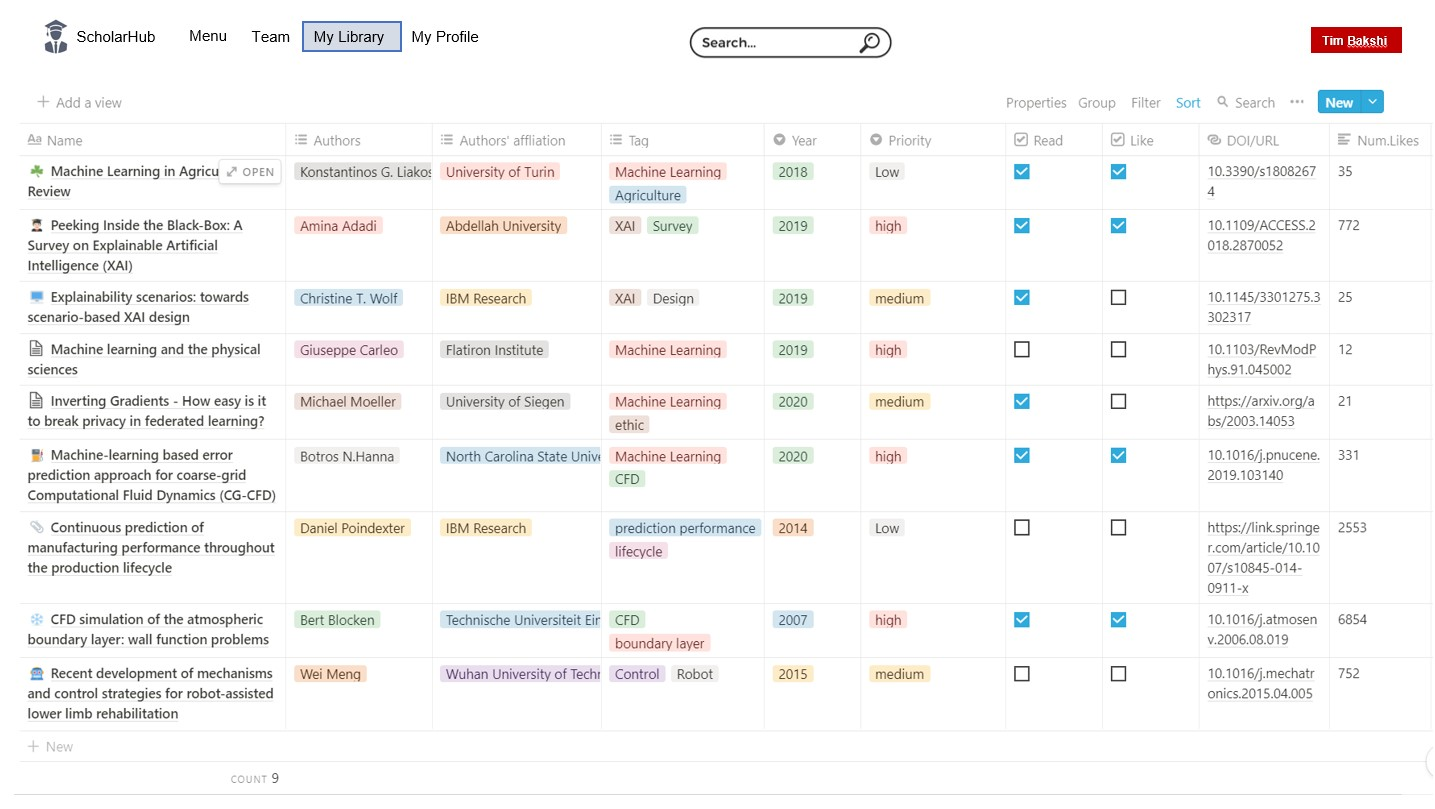
\includegraphics[width=\textwidth]{./img/UI My Library.jpg}
	\caption{My Library UI}
	\label{My Library UI}
\end{figure*}

\textbf {My Profile:} This page allows users to edit and show their profile cards. It contains the following information: Roles in the group, Address, Email, Mobile number, Personal web address, Resume or other attached document file and tags for showing research interest. Personal headshot photos can be uploaded and shown on the top for others’ recognition.

\begin{figure*}[htp]
	\centering
	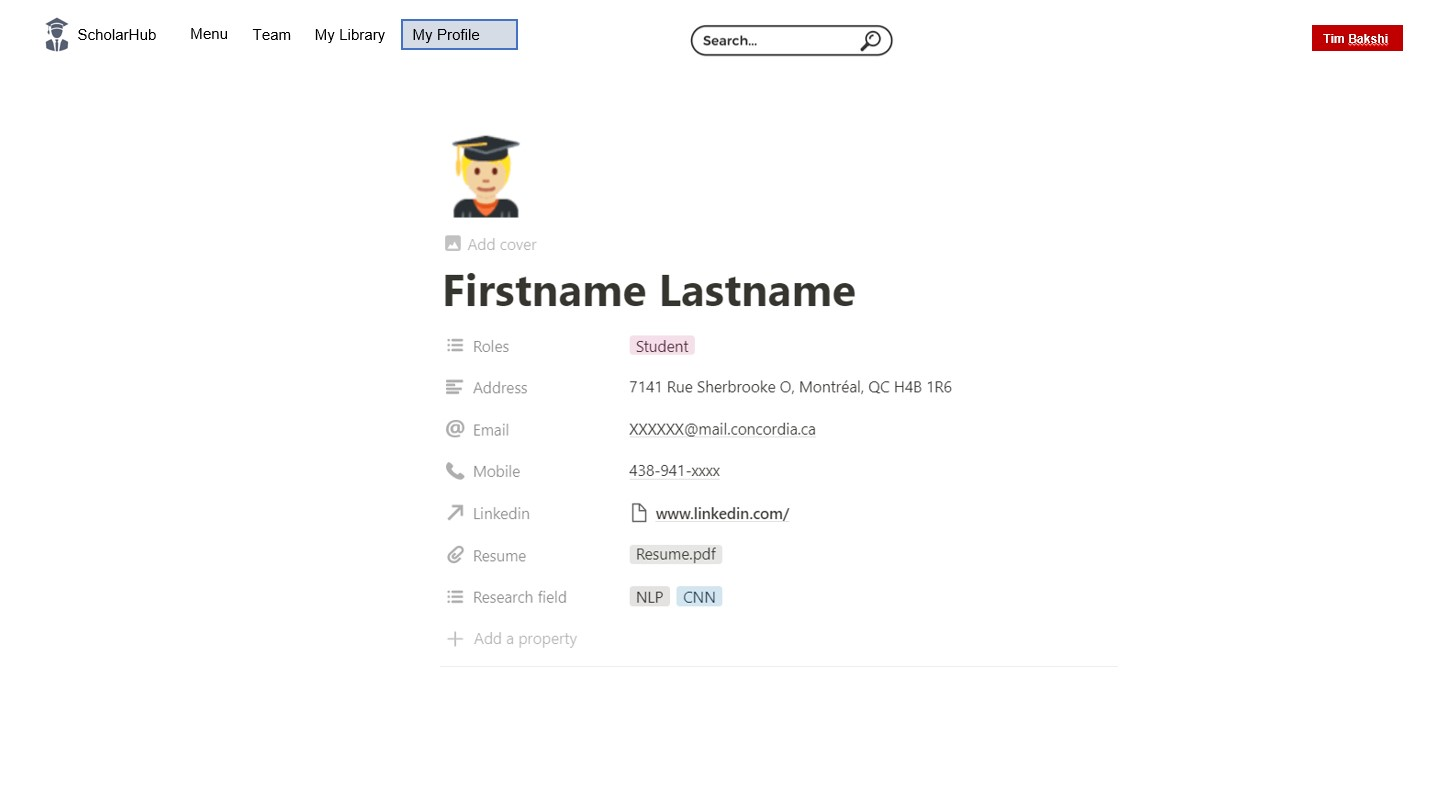
\includegraphics[width=\textwidth]{./img/UI my profile.jpg}
	\caption{My Profile UI}
	\label{my profile UI}
\end{figure*}

\textbf {Team:} The team function is the core of the ICDE system and is to share literature information with others. On the left side, the joined team is listed. If the user wants to join another new team or create a team, it would be just a simple click on the plus sign. Then, the pop-up window will request a team ID and password. The funder of a team can edit passwords. The information of team members will be listed in the table. Including the information about Name, Role, Stage position and so on. It is automatically extracted from their individual profile. Therefore, users can easily get the teammate’s contact information. By clicking the “activity”, the recently recorded activities will show by timeline. Also, the paper that the teammates liked will be listed on the right side for user to read.

\begin{figure*}[htp]
	\centering
	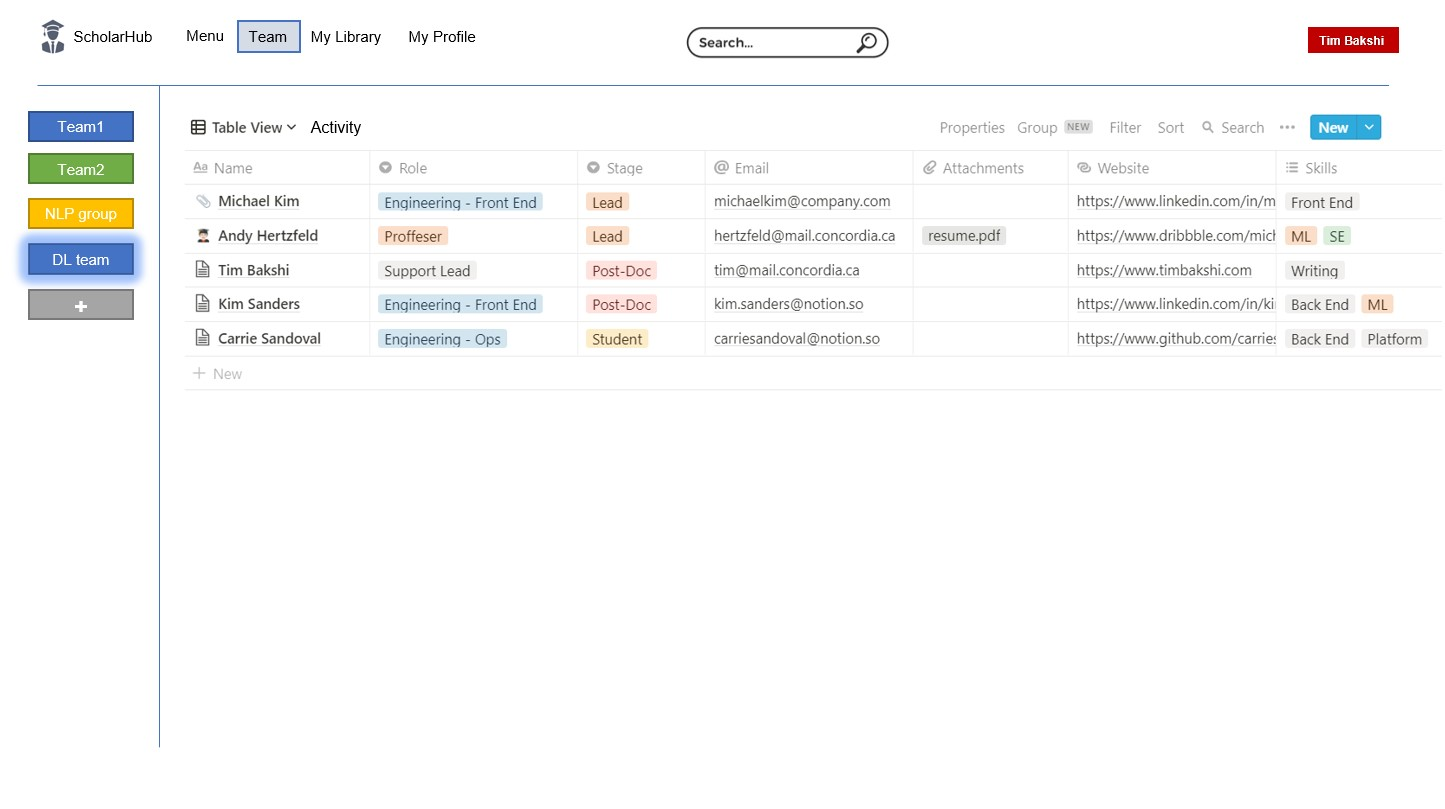
\includegraphics[width=\textwidth]{./img/UI teamlist.jpg}
	\caption{Team List UI}
	\label{teamlist UI}
\end{figure*}

\begin{figure*}[htp]
	\centering
	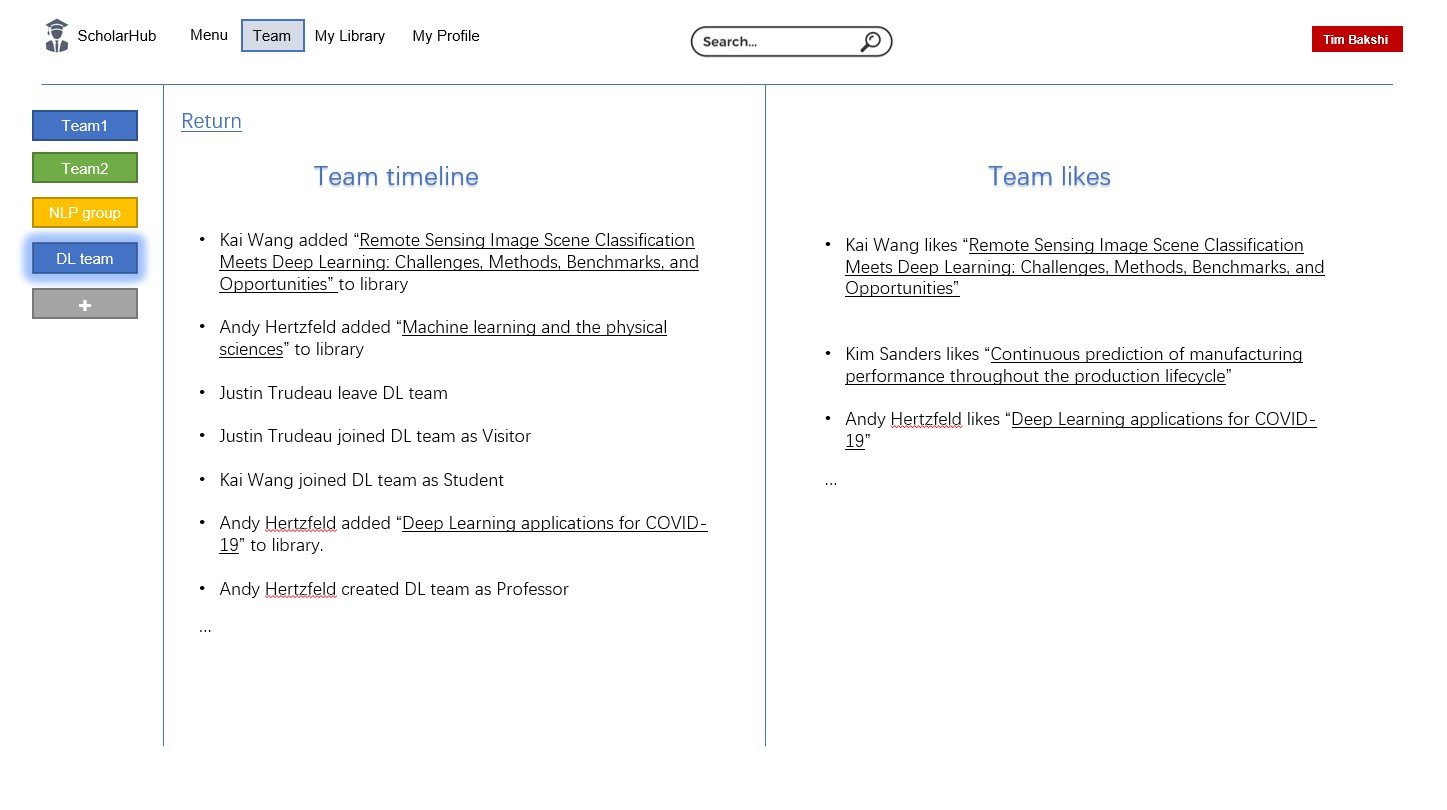
\includegraphics[width=\textwidth]{./img/UITeamactivity.jpg}
	\caption{Team Activity UI}
	\label{Teamactivity UI}
\end{figure*}